\chapter{\texorpdfstring{Algebras of $\PaB$}{Algebras of PaB}}
\lhead{\emph{algebras of $\PaB$}}
\section{Braided Monoidal Categories}
\begin{definition}[monoidal category]
	A category $\sC$ with a bifunctor $-\otimes-:\sC\times\sC\to\sC$ (the monoidal, or tensor product), unit object $\mathbf{1}$, and natural isomorphisms
	\begin{align}
		&\alpha:(-\otimes-)\otimes-\Rightarrow-\otimes(-\otimes-)\\
		&\lambda:\mathbf{1}\otimes-\Ra\id_\sC & \rho:-\otimes\mathbf{1}\Ra\id_{sC}
	\end{align}
	 respectively called the associator, left unitor, right unitor, is \emph{monoidal} if when we write $\otimes$ to act componentwise on natural transformations,
	\begin{enumerate}
	\item the triangle identity is satisfied, i.e. $\rho\otimes\id_\sC=(\id_\sC\otimes\lambda)\circ\alpha$
	\item the pentagon identity holds, i.e. for all $w,x,y,z\in\Obj(\sC)$, the following diagram commutes
	

\tikzset{every picture/.style={line width=0.75pt}} %set default line width to 0.75pt        
\[
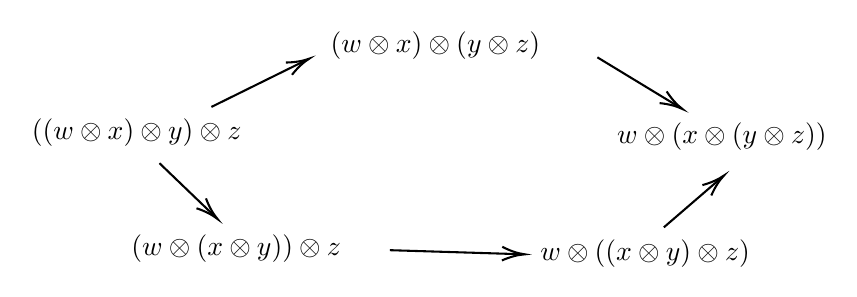
\begin{tikzpicture}[x=0.75pt,y=0.75pt,yscale=-1,xscale=1]
%uncomment if require: \path (0,497); %set diagram left start at 0, and has height of 497

%Straight Lines [id:da8091689343428804] 
\draw    (162,295.1) -- (207.41,272.69) ;
\draw [shift={(209.2,271.8)}, rotate = 153.73] [color={rgb, 255:red, 0; green, 0; blue, 0 }  ][line width=0.75]    (10.93,-3.29) .. controls (6.95,-1.4) and (3.31,-0.3) .. (0,0) .. controls (3.31,0.3) and (6.95,1.4) .. (10.93,3.29)   ;
%Straight Lines [id:da5599598183630712] 
\draw    (348,271.2) -- (387.29,295.06) ;
\draw [shift={(389,296.1)}, rotate = 211.27] [color={rgb, 255:red, 0; green, 0; blue, 0 }  ][line width=0.75]    (10.93,-3.29) .. controls (6.95,-1.4) and (3.31,-0.3) .. (0,0) .. controls (3.31,0.3) and (6.95,1.4) .. (10.93,3.29)   ;
%Straight Lines [id:da8391035848401762] 
\draw    (137,322.2) -- (163.56,347.71) ;
\draw [shift={(165,349.1)}, rotate = 223.85] [color={rgb, 255:red, 0; green, 0; blue, 0 }  ][line width=0.75]    (10.93,-3.29) .. controls (6.95,-1.4) and (3.31,-0.3) .. (0,0) .. controls (3.31,0.3) and (6.95,1.4) .. (10.93,3.29)   ;
%Straight Lines [id:da28460978615375354] 
\draw    (248,364.1) -- (311,366.04) ;
\draw [shift={(313,366.1)}, rotate = 181.76] [color={rgb, 255:red, 0; green, 0; blue, 0 }  ][line width=0.75]    (10.93,-3.29) .. controls (6.95,-1.4) and (3.31,-0.3) .. (0,0) .. controls (3.31,0.3) and (6.95,1.4) .. (10.93,3.29)   ;
%Straight Lines [id:da9551788148488187] 
\draw    (380,353.1) -- (407.49,329.41) ;
\draw [shift={(409,328.1)}, rotate = 139.24] [color={rgb, 255:red, 0; green, 0; blue, 0 }  ][line width=0.75]    (10.93,-3.29) .. controls (6.95,-1.4) and (3.31,-0.3) .. (0,0) .. controls (3.31,0.3) and (6.95,1.4) .. (10.93,3.29)   ;

% Text Node
\draw (74,299.4) node [anchor=north west][inner sep=0.75pt]    {$(( w\otimes x) \otimes y) \otimes z$};
% Text Node
\draw (218,257.4) node [anchor=north west][inner sep=0.75pt]    {$( w\otimes x) \otimes ( y\otimes z)$};
% Text Node
\draw (356,301.4) node [anchor=north west][inner sep=0.75pt]    {$w\otimes ( x\otimes ( y\otimes z))$};
% Text Node
\draw (122,355.4) node [anchor=north west][inner sep=0.75pt]    {$( w\otimes ( x\otimes y)) \otimes z$};
% Text Node
\draw (319,357.4) node [anchor=north west][inner sep=0.75pt]    {$w\otimes (( x\otimes y) \otimes z)$};


\end{tikzpicture}
\]
	or as natural transformations, $\alpha\circ\alpha=(\id_\sC\otimes\alpha)\circ\alpha\circ(\alpha\otimes\id_\sC)$
	\end{enumerate}
\end{definition}

A monoidal category is \emph{strict} if the components of the associator and unitors are identity morphisms.
\begin{definition}[braided monoidal category] \label{braidedMonoidalCategory}
	If $(\sC,\otimes,\mathbf{1},\alpha,\lambda,\rho)$ is a monoidal category with a natural isomorphism $\beta_{x,y}:x\otimes y\to y\otimes x$, then it is \emph{braided} if it satisfies the hexagon identities, i.e. the following diagrams commute
	\[
\begin{tikzcd}
	% https://tikzcd.yichuanshen.de/#N4Igdg9gJgpgziAXAbVABwnAlgFyxMJZABgBpiBdUkANwEMAbAVxiRAAoAPAHW4jwC28AAQBPAJS9+WIXGEAvEAF9S6TLnyEUARnJVajFmx59B8dqKlm588ctUgM2PASIAmPdXrNWiDpdMZEVsrILlOezVnTSIybX1vIz8LUNlhTklAtMUVKI1XHVJ4r0NfEADpWS5U4Ltcx3UXLWQPYoMfNgrrdnka8Lr9GCgAc3giUAAzACcIASQyEBwIJABmEo6-XgAjGBw6Pt4sKAB9XjgAYRBqBjodhgAFRpi-BhgJnEiQadn56iWkXTtJIgXiMNAACzoVxANzuj2iBRhbw+9W+c0QgP+iA8QLK212UOutxgDyeiNe70+aKQOKxAFZ1sDQQwIYSYcTSQitEjKaiZui1otlogACyMvHcMGQ6Gwknw-LcikohzU0V-YUM9lwsmK5HQxISo6nbgXA7cHZ7ZQUJRAA
(x\otimes y)\otimes z \arrow[d, "\beta\otimes\id_\sC"] \arrow[r, "\alpha"] & x\otimes(y\otimes z) \arrow[r, "\beta"]               & (y\otimes z)\otimes x \arrow[d, "\alpha"] \\
(y\otimes x)\otimes z \arrow[r, "\alpha"]                                  & y\otimes(x\otimes z) \arrow[r, "\id_\sC\otimes\beta"] & y\otimes(z\otimes x)                     
\end{tikzcd}\]
	\[
\begin{tikzcd}
	% https://tikzcd.yichuanshen.de/#N4Igdg9gJgpgziAXAbVABwnAlgFyxMJZABgBpiBdUkANwEMAbAVxiRAA8AdTiPAW3gAKAJ7deWAXAAEALwCUIAL6l0mXPkIoAjOSq1GLNoK49+8KcLliz0mUpUgM2PASIAmXdXrNWiEDOsJIRNxSQsFZVVnDXdSLT1vQz9BANMg6XYrNLDheyj1VxQyeK8DXw5AyRTK80s8xzUXTWQdEv0fIxCbWSzQ2qU9GCgAc3giUAAzACcIPiQyEBwIJB12pJBuRjQACzoAPWAAWi1FeunZleolpA818u4AIxgcOjOZucRb68QAZlKOvybBg7fZHE5vC6IBbfAAs-3W3CwUAA+tw4ABhGpwR7PV6REDnD5wxbLRAAVnh904W12B2Op3xhKQFJJSD+dzYOJeWMRKLR6IGiiAA
x\otimes(y\otimes z) \arrow[r, "\alpha^{-1}"] \arrow[d, "\id_\sC\otimes\beta"] & (x\otimes y)\otimes z \arrow[r, "\beta"]               & z\otimes(x\otimes y) \arrow[d, "\alpha^{-1}"] \\
x\otimes(z\otimes y) \arrow[r, "\alpha^{-1}"]                                  & (x\otimes z)\otimes y \arrow[r, "\beta\otimes\id_\sC"] & (z\otimes x)\otimes y                        
\end{tikzcd}\]
\end{definition}

We will now build up to Mac Lane's Coherence Theorem
\begin{definition}[monoidal functor, or strong monoidal functor at nLab]
	Suppose $(\sC,\otimes,\mathbf{1},\alpha,\lambda,\rho)$, and $(\sC',\otimes',\mathbf{1}',\alpha',\lambda',\rho')$, are monoidal categories, then a monoidal functor consists of a functor $F:\sC\to\sC'$ such that $\mathbf{1'}\cong F(\mathbf{1})$, and a natural isomorphism $m:F(-)\otimes F(-)\to F(-\otimes-)$ such that the following diagram commutes
	\[\begin{tikzcd}
		% https://tikzcd.yichuanshen.de/#N4Igdg9gJgpgziAXAbVABwnAlgFyxMJZABgBpiBdUkANwEMAbAVxiRAAoAxdgDQEoAOgIh4AtvAAE3AJp9BwsZO4AtPiAC+pdJlz5CKMgEYqtRizbceQkVnFwJs64vsq1m7djwEiZAEwn6ZlZEEG5eJ1tJRwVI+1UNLRAMTz0iQ1J-akDzEMsIu3ZpfMlVN0Tk3W8UdMoss2DQ3nkbAplm5yl2UoSPSv1kdOM6oIsm4pdC8Yl49RMYKABzeCJQADMAJwhRJDIQHAgkdNMRkNFxoSwoAH0hOABhHpANrcPqfaRfYZyQbfcnze2iE+ewOiAAzF8GtwhIw0AALOhlNYAnZvUEAFkhbBhDHhdAA5I9noDMSCkABWLEhC7XW53Ka-RLEilopAQ47fX4UdRAA
(F(X)\otimes F(Y))\otimes F(Z) \arrow[d, "m\otimes\id_\sC"] \arrow[r, "\alpha'"] & F(X)\otimes(F(Y)\otimes F(Z)) \arrow[d, "\id_\sC\otimes m"] \\
F(X\otimes Y)\otimes F(Z) \arrow[d, "m"]                                         & F(X)\otimes F(Y\otimes Z) \arrow[d, "m"]                    \\
F((X\otimes Y)\otimes Z) \arrow[r, "F(\alpha)"]                                  & F(X\otimes(Y\otimes Z))                                    
\end{tikzcd}\]
\end{definition}
A monoidal functor that happens to be an equivalence of categories is called an \emph{equivalence of monoidal categories}.
\begin{theorem}[Mac Lane's Strictness Theorem]
	For any monoidal category\\
	$(\sC,\otimes,\mathbf{1},\alpha,\lambda,\rho)$, there exists a \emph{strict} monoidal category $(\sC',\otimes',\mathbf{1}',\alpha',\lambda',\rho')$ and an equivalence of monoidal categories $L:\sC\to\sC'$.
\end{theorem}
\begin{proof}
	see pg. 20 of \cite{Etingof} from the 2009 lecture notes to "Topics in Lie Theory".
	% Let $\sC'$ be pairs $(F,c)$ where $F$ is an endofunctor of $\sC$, and $c:F(-)\otimes\id_\sC\to F(-\otimes\id_\sC)$ is a natural isomorphism. Then $\sC'$ is strict, and we can construct an equivalence of monoidal categories $L:\sC\to\sC'$ by left multiplication:
	% \begin{enumerate}
	% 	\item For all $X\in\Obj(\sC)$, $L(X)\defeq X\otimes-$.
	% 	\item For morphisms $f$ in $\sC$, $L(f)\defeq f\otimes-$.
	% \end{enumerate}
\end{proof}
The next theorem is a corollary of Mac Lane's Strictness Theorem.
\begin{theorem}[Mac Lane's Coherence Theorem] \label{MacLaneCoherenceThm}
	Suppose $P$ and $P'$ are parenthesizations of $X_1\otimes\cdots\otimes X_n$ with arbitrary insertions of $\mathbf{1}$, and $f,g:P\to P'$ are isomorphisms built by composing associator and unitor components, then $f=g$.
\end{theorem}
\begin{proof}
	see pg. 1 of \cite{Etingof_2009}
\end{proof}

\section{\texorpdfstring{The Operad $\PaB$ of Parenthesized Braids}{The Operad PaB of Parenthesized Braids}}
Operads are an unbiased way of keeping track of $n$-ary operations and how they compose. The "elements" of $P(n)$, we imagine to be corollas, i.e., rooted trees of depth 1 with $n+1$ half-edges. We can treat $\otimes$ in this "unbiased" way (i.e. ignoring how products are parenthesized, and products with units) because of Mac Lane's Coherence Theorem \ref{MacLaneCoherenceThm}.
\begin{definition}[planar operad, symmetric operad]
	A \emph{planar operad} $P$ in a monoidal category $(\sC,\otimes,\mathbf{1},a,l,r)$
	% $(\sC,\otimes,\mathbf{1},a,l,r,b)$ (i.e. a braided monoidal category such that $b\circ b=\id_\sC$)
	is a collection of objects $\left\{ P(n) \right\}_n$, with operadic composition
	\[c_{m;n_1,\cdots,n_m}:P(m)\otimes P(n_1)\otimes\cdots\otimes P(n_m)\to P(n_1+\cdots+n_m)\]
	such that 1. and 2. of following are satisfied. If each object $P(n)$ has a right $S_n$-action ($S_n$ being the $n$th symmetric group), and 3. is staisfied, then $P$ is a \emph{symmetric operad}, which is what "operad" refers to from now on.
	\begin{enumerate}
		\item Associativity: if
			\begin{enumerate}
			\item $\sum_{j=1}^{m_i}n_{i_j}=n_i$ for each $1\le i\le k$,
			\item $\sum_{i=1}^{k}n_i=l$,
			\item $\sum_{i=1}^k m_i=m$,
			\end{enumerate}
		then the following commutes
\[\begin{tikzcd}
	% https://q.uiver.app/#q=WzAsNixbMCwwLCJQKGspXFxvdGltZXNcXGJpZ290aW1lc197aT0xfV5rXFxsZWZ0KFAobV9pKVxcb3RpbWVzXFxiaWdvdGltZXNfe2o9MX1ee21faX1QKG5fe2lfan0pXFxyaWdodCkiXSxbMCwxLCJQKGspXFxvdGltZXNcXGJpZ290aW1lc197aT0xfV5rUFxcbGVmdChuX2lcXHJpZ2h0KSJdLFsyLDIsIlAobCkiXSxbMiwwLCJcXGxlZnQoUChrKVxcb3RpbWVzXFxiaWdvdGltZXNfe2k9MX1ee2t9UChtX2kpXFxyaWdodClcXG90aW1lc1xcbGVmdChcXGJpZ290aW1lc197aT0xfV5rXFxiaWdvdGltZXNfe2o9MX1ee21faX1QKG5fe2lfan0pXFxyaWdodCkiXSxbMiwxLCJQKG0pXFxvdGltZXNcXGxlZnQoXFxiaWdvdGltZXNfe2k9MX1ea1xcYmlnb3RpbWVzX3tqPTF9XnttX2l9UChuX3tpX2p9KVxccmlnaHQpIl0sWzAsMiwiUChsKSJdLFswLDEsIlxcaWRfXFxzQ1xcb3RpbWVzXFxiaWdvdGltZXNfe2k9MX1ea2Nfe21faTtuX3tpXzF9LFxcY2RvdHMsbl97aV97bV9pfX19Il0sWzAsMywiXFxjb25nIiwyXSxbMyw0LCJcXGNpcmNfe2s7bV8xLFxcY2RvdHMsbV9rfVxcb3RpbWVzXFxpZF9cXHNDXntcXG90aW1lcyBtfSIsMl0sWzQsMiwiXFxjaXJjX3ttO25fezFfMX0sXFxjZG90cyxuX3trX3sobV9rKX19fSIsMl0sWzEsNSwiXFxjaXJjX3trO25fMSxcXGNkb3RzLG5fa30iXSxbNSwyLCI9Il1d
	{P(k)\otimes\bigotimes_{i=1}^k\left(P(m_i)\otimes\bigotimes_{j=1}^{m_i}P(n_{i_j})\right)} && {\left(P(k)\otimes\bigotimes_{i=1}^{k}P(m_i)\right)\otimes\left(\bigotimes_{i=1}^k\bigotimes_{j=1}^{m_i}P(n_{i_j})\right)} \\
	{P(k)\otimes\bigotimes_{i=1}^kP\left(n_i\right)} && {P(m)\otimes\left(\bigotimes_{i=1}^k\bigotimes_{j=1}^{m_i}P(n_{i_j})\right)} \\
	{P(l)} && {P(l)}
	\arrow["\cong"', from=1-1, to=1-3]
	\arrow["{\id_\sC\otimes\bigotimes_{i=1}^kc_{m_i;n_{i_1},\cdots,n_{i_{m_i}}}}", from=1-1, to=2-1]
	\arrow["{\circ_{k;m_1,\cdots,m_k}\otimes\id_\sC^{\otimes m}}"', from=1-3, to=2-3]
	\arrow["{\circ_{k;n_1,\cdots,n_k}}", from=2-1, to=3-1]
	\arrow["{\circ_{m;n_{1_1},\cdots,n_{k_{(m_k)}}}}"', from=2-3, to=3-3]
	\arrow["{=}", from=3-1, to=3-3]
\end{tikzcd}\]
		\item Unit: there exists a map $e:\mathbf{1}\to P(1)$ such that the following hold for all $n$
\[\begin{tikzcd}
	% https://q.uiver.app/#q=WzAsNCxbMCwwLCJQKG4pIl0sWzEsMCwiXFxtYXRoYmZ7MX1cXG90aW1lcyBQKG4pIl0sWzIsMCwiUCgxKVxcb3RpbWVzIFAobikiXSxbMywwLCJQKG4pIl0sWzAsMSwiXFxsYW1iZGFeey0xfSJdLFsxLDIsImVcXG90aW1lc1xcaWRfXFxzQyJdLFsyLDMsIlxcY2lyY197MTtufSJdLFswLDMsIj0iLDIseyJjdXJ2ZSI6Mn1dXQ==
	{P(n)} & {\mathbf{1}\otimes P(n)} & {P(1)\otimes P(n)} & {P(n)}
	\arrow["{\lambda^{-1}}", from=1-1, to=1-2]
	\arrow["{=}"', curve={height=12pt}, from=1-1, to=1-4]
	\arrow["{e\otimes\id_\sC}", from=1-2, to=1-3]
	\arrow["{\circ_{1;n}}", from=1-3, to=1-4]
\end{tikzcd}\]
\[\begin{tikzcd}
	% https://q.uiver.app/#q=WzAsNCxbMCwwLCJQKG4pIl0sWzEsMCwiUChuKVxcb3RpbWVzXFxtYXRoYmZ7MX1ee1xcb3RpbWVzIG59Il0sWzIsMCwiUChuKVxcb3RpbWVzIFAoMSlee1xcb3RpbWVzIG59Il0sWzMsMCwiUChuKSJdLFswLDEsIihcXHJob157LTF9KV57XFxjaXJjIG59Il0sWzEsMiwiXFxpZF9cXHNDXFxvdGltZXMgZV57XFxvdGltZXMgbn0iXSxbMiwzLCJcXGNpcmNfe247MSxcXGNkb3RzLDF9Il0sWzAsMywiPSIsMix7ImN1cnZlIjoyfV1d
	{P(n)} & {P(n)\otimes\mathbf{1}^{\otimes n}} & {P(n)\otimes P(1)^{\otimes n}} & {P(n)}
	\arrow["{(\rho^{-1})^{\circ n}}", from=1-1, to=1-2]
	\arrow["{=}"', curve={height=12pt}, from=1-1, to=1-4]
	\arrow["{\id_\sC\otimes e^{\otimes n}}", from=1-2, to=1-3]
	\arrow["{\circ_{n;1,\cdots,1}}", from=1-3, to=1-4]
\end{tikzcd}\]
		\item Equivariance: the right action $-\cdot\sigma:P(n)\to P(n)$ of $\sigma\in S_n$ on $P(n)$ is given by $\sigma$ permuting the $n$ inputs of each "element" of $P(n)$, so that on operadic composition maps, we have
		\[\circ_{n;m_1,\cdots,m_n}\circ(-\cdot\sigma) = \circ_{n;m_{\sigma^{-1}(1)},\cdots,m_{\sigma^{-1}(n)}},\]
		then equivariance is the condition that the following commutes
\[\begin{tikzcd}
	% https://q.uiver.app/#q=WzAsNCxbMCwwLCJQKG4pXFxvdGltZXNcXGJpZ290aW1lc197aT0xfV5uUChtX2kpIl0sWzAsMSwiUChuKVxcb3RpbWVzXFxiaWdvdGltZXNfe2k9MX1eblAobV9pKSJdLFsxLDEsIlAobV8xK1xcY2RvdHMrbV9uKSJdLFsxLDAsIlAobilcXG90aW1lc1xcYmlnb3RpbWVzX3tpPTF9Xm5QKG1fe1xcc2lnbWFeey0xfShpKX0pIl0sWzAsMSwiLVxcY2RvdFxcc2lnbWFcXG90aW1lc1xcaWRfXFxzQ157XFxvdGltZXMgbn0iXSxbMSwyLCJcXGNpcmNfe247bV8xLFxcY2RvdHMsbV9ufSJdLFswLDMsIlxcaWRfXFxzQ1xcb3RpbWVzKC0pXFxzaWdtYSIsMl0sWzMsMiwiXFxjaXJjX3tuO21fe1xcc2lnbWFeey0xfSgxKX0sXFxjZG90cyxtX3tcXHNpZ21hXnstMX0obil9fSIsMl1d
	{P(n)\otimes\bigotimes_{i=1}^nP(m_i)} & {P(n)\otimes\bigotimes_{i=1}^nP(m_{\sigma^{-1}(i)})} \\
	{P(n)\otimes\bigotimes_{i=1}^nP(m_i)} & {P(m_1+\cdots+m_n)}
	\arrow["{\id_\sC\otimes(-)\sigma}"', from=1-1, to=1-2]
	\arrow["{-\cdot\sigma\otimes\id_\sC^{\otimes n}}", from=1-1, to=2-1]
	\arrow["{\circ_{n;m_{\sigma^{-1}(1)},\cdots,m_{\sigma^{-1}(n)}}}"', from=1-2, to=2-2]
	\arrow["{\circ_{n;m_1,\cdots,m_n}}", from=2-1, to=2-2]
\end{tikzcd}\]
(where $(-)\sigma$ is the isomorphism given by $\sigma$ permuting the $n$ factors of $\bigotimes_{i=1}^nP(m_i)$)
	\end{enumerate}
\end{definition}
\begin{example}[the endomorphism operad]
	If $(\sC,\otimes,\mathbf{1},\alpha,\lambda,\rho,\beta)$ is a braided monoidal category, then $\End(\sC) $
\end{example}
% \begin{definition}[braided operad]
% 	This is theorem 4.3.6 from \cite{Yau_2021} reduced to the 1-coloured case.
% \end{definition}
% \begin{remark}
% 	Symmetric operads are special cases of braided operads, where $b\in B(n)$ acts via its underlying permutation $\bar{b}$.
% \end{remark}
\begin{definition}[operad morphism]
	A morphism $f:P\to Q$ of operads is a collection of maps $\left\{ f_n:P(n)\to Q(n) \right\}_{n}$ such that
	\begin{enumerate}
		\item The unit is preserved, i.e. $f_1:P(1)\to Q(1)$ satisfies $f_1\circ e^P=e^Q$.
		\item Composition is preserved, i.e. for all $k,n_1,\cdots,n_k\in\bN_{\ge1}$ with $l=\sum_{i=1}^kn_i$, the following commutes
		\[\begin{tikzcd}
			% https://q.uiver.app/#q=WzAsNCxbMSwwLCJRKGspXFxvdGltZXNcXGJpZ290aW1lc197aT0xfV5rUShuX2kpIl0sWzEsMSwiUShsKSJdLFswLDEsIlAobCkiXSxbMCwwLCJQKGspXFxvdGltZXNcXGJpZ290aW1lc197aT0xfV5rUChuX2kpIl0sWzMsMiwiXFxjaXJjXlBfe2s7bl8xLFxcY2RvdHMsbl9rfSJdLFswLDEsIlxcY2lyY15RX3trO25fMSxcXGNkb3RzLG5fa30iXSxbMiwxLCJmX2wiLDJdLFszLDAsImZfa1xcb3RpbWVzXFxiaWdvdGltZXNfe2k9MX1ea2Zfe25faX0iLDJdXQ==
			{P(k)\otimes\bigotimes_{i=1}^kP(n_i)} & {Q(k)\otimes\bigotimes_{i=1}^kQ(n_i)} \\
			{P(l)} & {Q(l)}
			\arrow["{f_k\otimes\bigotimes_{i=1}^kf_{n_i}}"', from=1-1, to=1-2]
			\arrow["{\circ^P_{k;n_1,\cdots,n_k}}", from=1-1, to=2-1]
			\arrow["{\circ^Q_{k;n_1,\cdots,n_k}}", from=1-2, to=2-2]
			\arrow["{f_l}"', from=2-1, to=2-2]
		\end{tikzcd}\]
		\item The $S_n$-actions are preserved, i.e. for all $n\in\bN_{\ge1}$, $\sigma\in S_n$, $f\circ(-\cdot^P\sigma)=(-\cdot^Q\sigma)\circ f$.
	\end{enumerate}
\end{definition}